%%%%%%%%%%%%%%%%%%%%%%%%%%%%%%%%%%%%%%%%%
% Jacobs Landscape Poster
% LaTeX Template
% Version 1.1 (14/06/14)
%
% Created by:
% Computational Physics and Biophysics Group, Jacobs University
% https://teamwork.jacobs-university.de:8443/confluence/display/CoPandBiG/LaTeX+Poster
% 
% Further modified by:
% Nathaniel Johnston (nathaniel@njohnston.ca)
%
% This template has been downloaded from:
% http://www.LaTeXTemplates.com
%
% License:
% CC BY-NC-SA 3.0 (http://creativecommons.org/licenses/by-nc-sa/3.0/)
%
%%%%%%%%%%%%%%%%%%%%%%%%%%%%%%%%%%%%%%%%%

%----------------------------------------------------------------------------------------
%	PACKAGES AND OTHER DOCUMENT CONFIGURATIONS
%----------------------------------------------------------------------------------------

\documentclass[xcolor=table]{beamer}

\usefonttheme{default}

\usepackage[scale=0.9]{beamerposter} % Use the beamerposter package for laying out the poster
\usepackage{adjustbox}
\usepackage{threeparttable} % Use footnote
\usepackage{multirow}




\usetheme{confposter} % Use the confposter theme supplied with this template

\setbeamercolor{headline}{fg=Maroon, bg=white}
\setbeamercolor{block title}{fg=Maroon,bg=white} % Colors of the block titles
\setbeamercolor{block body}{fg=black,bg=white} % Colors of the body of blocks
\setbeamercolor{block alerted title}{fg=Maroon,bg=Maroon!10} % Colors of the highlighted block titles
\setbeamercolor{block alerted body}{fg=black,bg=Maroon!10} % Colors of the body of highlighted blocks


% Many more colors are available for use in beamerthemeconfposter.sty


%-----------------------------------------------------------
% Define the column widths and overall poster size
% To set effective sepwid, onecolwid and twocolwid values, first choose how many columns you want and how much separation you want between columns
% In this template, the separation width chosen is 0.024 of the paper width and a 4-column layout
% onecolwid should therefore be (1-(# of columns+1)*sepwid)/# of columns e.g. (1-(4+1)*0.024)/4 = 0.22
% Set twocolwid to be (2*onecolwid)+sepwid = 0.464
% Set threecolwid to be (3*onecolwid)+2*sepwid = 0.708

\newlength{\sepwid}
%\newlength{\onecolwid}
%\newlength{\twocolwid}
%\newlength{\threecolwid}
\setlength{\paperwidth}{48.5in} % A0 width: 46.8in
\setlength{\paperheight}{35in} % A0 height: 33.1in
\setlength{\sepwid}{0.01\paperwidth} % Separation width (white space) between columns
%\setlength{\onecolwid}{0.22\paperwidth} % Width of one column
%\setlength{\twocolwid}{0.464\paperwidth} % Width of two columns
%\setlength{\threecolwid}{0.708\paperwidth} % Width of three columns
\setlength{\topmargin}{-0.5in} % Reduce the top margin size
%-----------------------------------------------------------


\usepackage{graphicx}  % Required for including images

\usepackage{booktabs} % Top and bottom rules for tables
\usepackage{xcolor}


%----------------------------------------------------------------------------------------
%	TITLE SECTION 
%----------------------------------------------------------------------------------------

\title{Applying A Global Sensitivity Analysis Workflow to Improve the Computational Efficiencies in Physiologically-Based Pharmacokinetic Model} % Poster title

\author{Nan-Hung Hsieh$^1$, Weihsueh A. Chiu$^1$, Brad Reisfeld$^2$, Frederic Y. Bois$^3$} % Author(s)

\institute{
$^1$Department of Veterinary Integrative Biosciences ,Texas A\&M University, College Station, TX, USA\\
$^2$Chemical and Biological Engineering ,Colorado State University, Fort Collins, CO, USA\\
$^3$Models for Ecotoxicology and Toxicology Unit, Institut National de l'Environnement Industriel et des Risques, Verneuil en Halatte, France
} % Institution(s)



%----------------------------------------------------------------------------------------

\begin{document}

\addtobeamertemplate{block end}{}{\vspace*{0ex}} % White space under blocks
\addtobeamertemplate{block alerted end}{}{\vspace*{2ex}} % White space under highlighted (alert) blocks

\setlength{\belowcaptionskip}{0ex} % White space under figures
\setlength\belowdisplayshortskip{2ex} % White space under equations

\begin{frame}[t] % The whole poster is enclosed in one beamer frame

\begin{columns}[t] % The whole poster consists of three major columns, the second of which is split into two columns twice - the [t] option aligns each column's content to the top

\begin{column}{\sepwid}\end{column} % Empty spacer column


%%%%%%%%%%%%%%%%%%%%%%%%%%%%%%%%%%%%%%%%%%%%%%%%%%%
\begin{column}{0.25\paperwidth} % The first column
%
%
\begin{alertblock}{Motivations}
The population physiologically-based pharmacokinetic (PBPK) model usually constructed from dozens of parameters that are affected by uncertainties and can change the model output.
The complexity of PBPK model poses a challenge in estimating parameters due to many parameters being unidentifiable. 
To increase computational efficiency, the current approach is to fix known model parameters and only optimize the small subset of parameters. 
However, this method can lead to problems such as biased estimates for fitted parameters due to correlations/interactions with the fixed parameter. 
The purpose of this study is to propose a global sensitivity analysis (GSA) workflow which can 

\begin{itemize}
\item \textbf{Reduce the PBPK model parameters dimensionality}
\item \textbf{Reduce the computational burden without introducing bias}
\item \textbf{Mantain the reliability of parameter estimates and model performance}
\end{itemize}

\end{alertblock}

%----------------------------------------------------------------------------------------
%	INTRODUCTION
%----------------------------------------------------------------------------------------

\setbeamercolor{block alerted title}{fg=Maroon,bg=black!10} % Change the alert block title colors
\setbeamercolor{block alerted body}{fg=black,bg=white} % Change the alert block body colors
\setbeamercolor{block title}{fg=Maroon,bg=white} % Change the block title color

\begin{alertblock}{Workflow}
We applied our published PBPK model for testing, which can predict and characterize the absorption, distribution, metabolism, and excretion of acetaminophen (APAP) with two major metabolites of APAP-glucuronide and APAP-sulfate in humans \cite{Zurlinden}.
In our GSA workflow, we evaluated three variance-based GSA approach that can calculate both main and total effects as sensitivity indices \cite{McNally, Jansen, Owen}.
Moreover, we also applied the elementary effects method to compare the sensitivity indices from variance-based GSA approach and judge the reliability of each method. 
To understand the time-dependent variation of sensitivity index, we examine each index in 12-hours after APAP intake as GSA time points.
Finally, we compare the model performance (accuracy and precision) among the four different parameter settings.

\begin{figure}
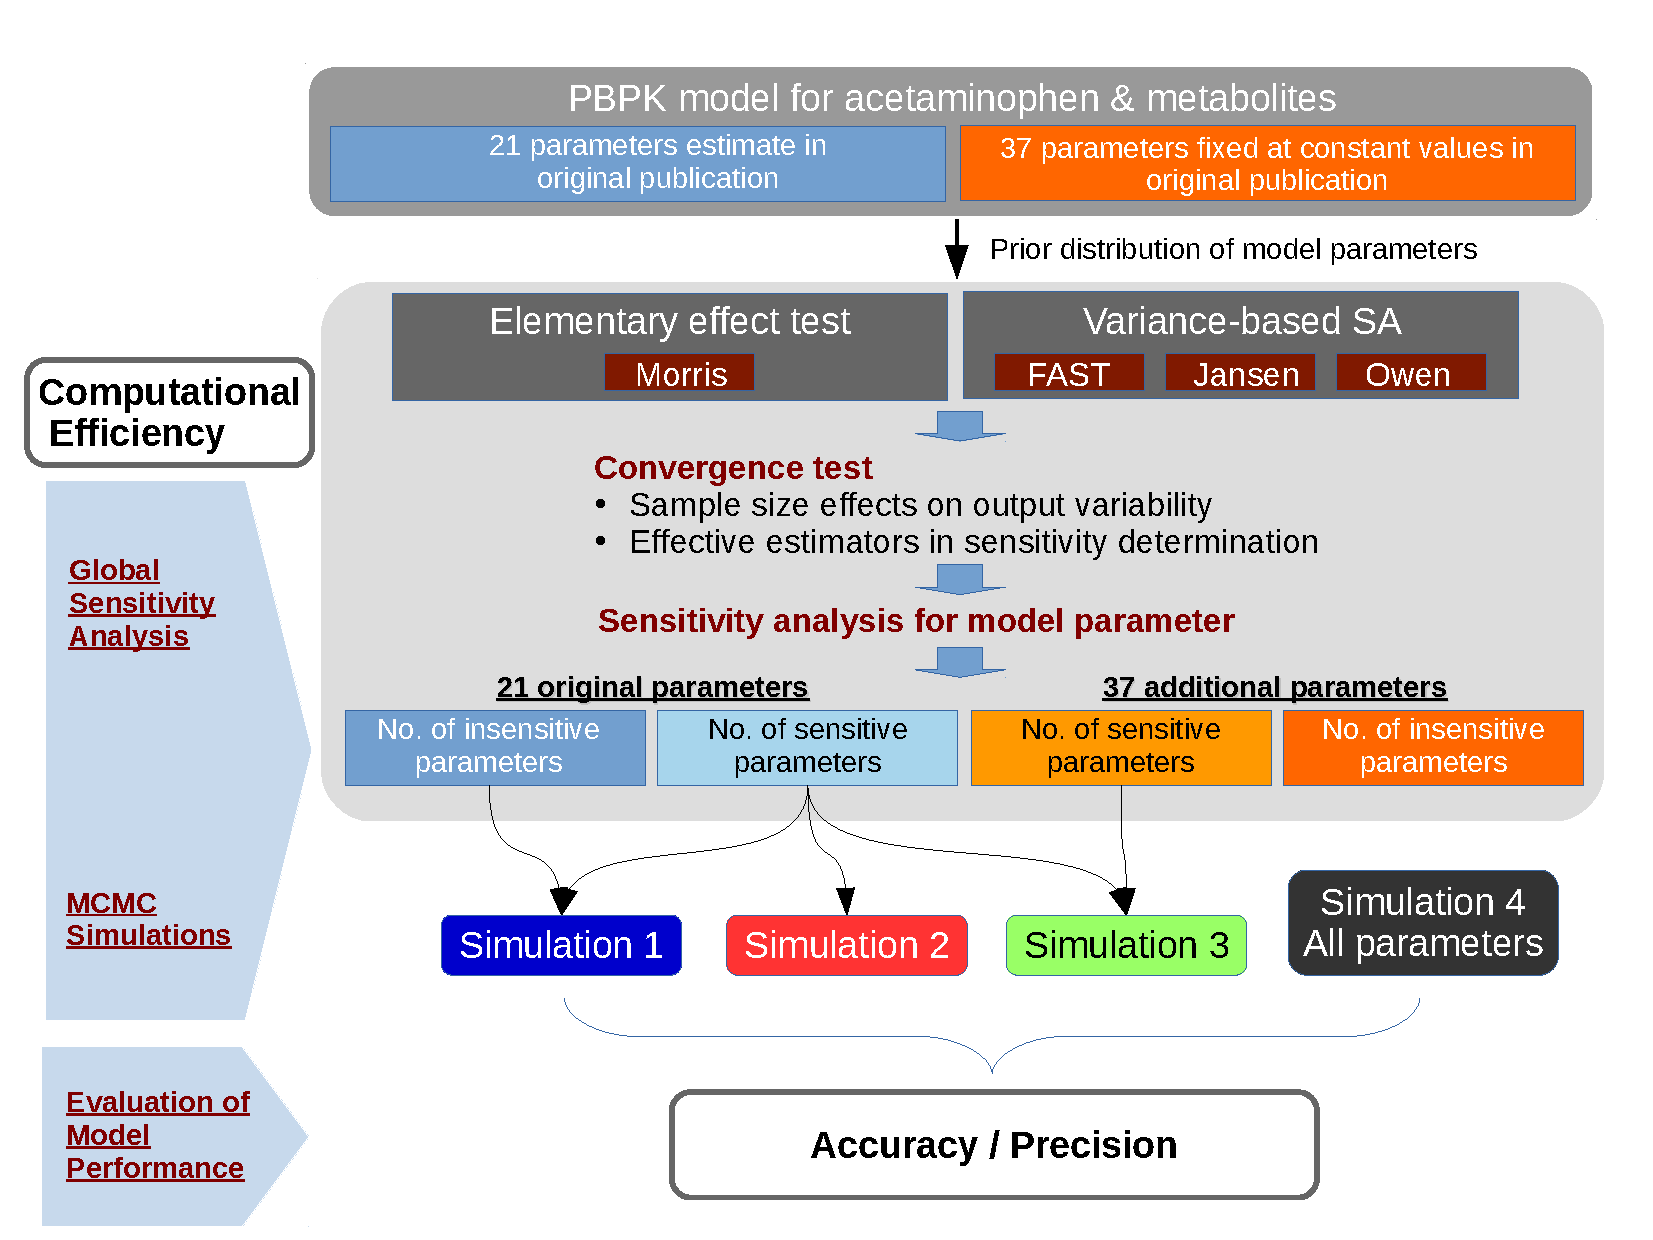
\includegraphics[width=0.9\linewidth]{fig0.pdf}
\caption{Schematic illustration of the GSA workflow with Bayesian population PBPK modelling}
\end{figure}

\end{alertblock}

\begin{alertblock}{Software and computing platform}
This study was fully conduct in open source environment. 
Statistical analysis and visualization results were carried out in R v3.4.0.
The GSA was performed with R "Sensitivity" package v1.15 \cite{Pujol17}. 
The MCMC simulations and setpoint analyses were conducted using MCSim v5.6 \cite{Bois09}.
Parallelizing computation was performed in high performance computing cluster with four chains in CentOS Linux distribution.

\vspace{10mm} %5mm vertical space

\noindent\begin{minipage}{0.85\textwidth}% adapt widths of minipages to your needs
\textbf{Source code}\\
\small{This poster was making by Latex-BeamerPoster.}\\
\small{All source code can find in the github repository: nanhung/GSAposter}\\
\end{minipage}%
\hfill%
\begin{minipage}{0.1\textwidth}

\includegraphics[width=1\linewidth]{QR}
\end{minipage}

\end{alertblock}

\end{column} % End of the first column


%%%%%%%%%%%%%%%%%%%%%%%%%%%%%%%%%%%%%%%%%%%%%%%%%
\begin{column}{0.23\paperwidth} % The 2nd column

\begin{block}{Convergence and Computation Time}
\begin{figure}
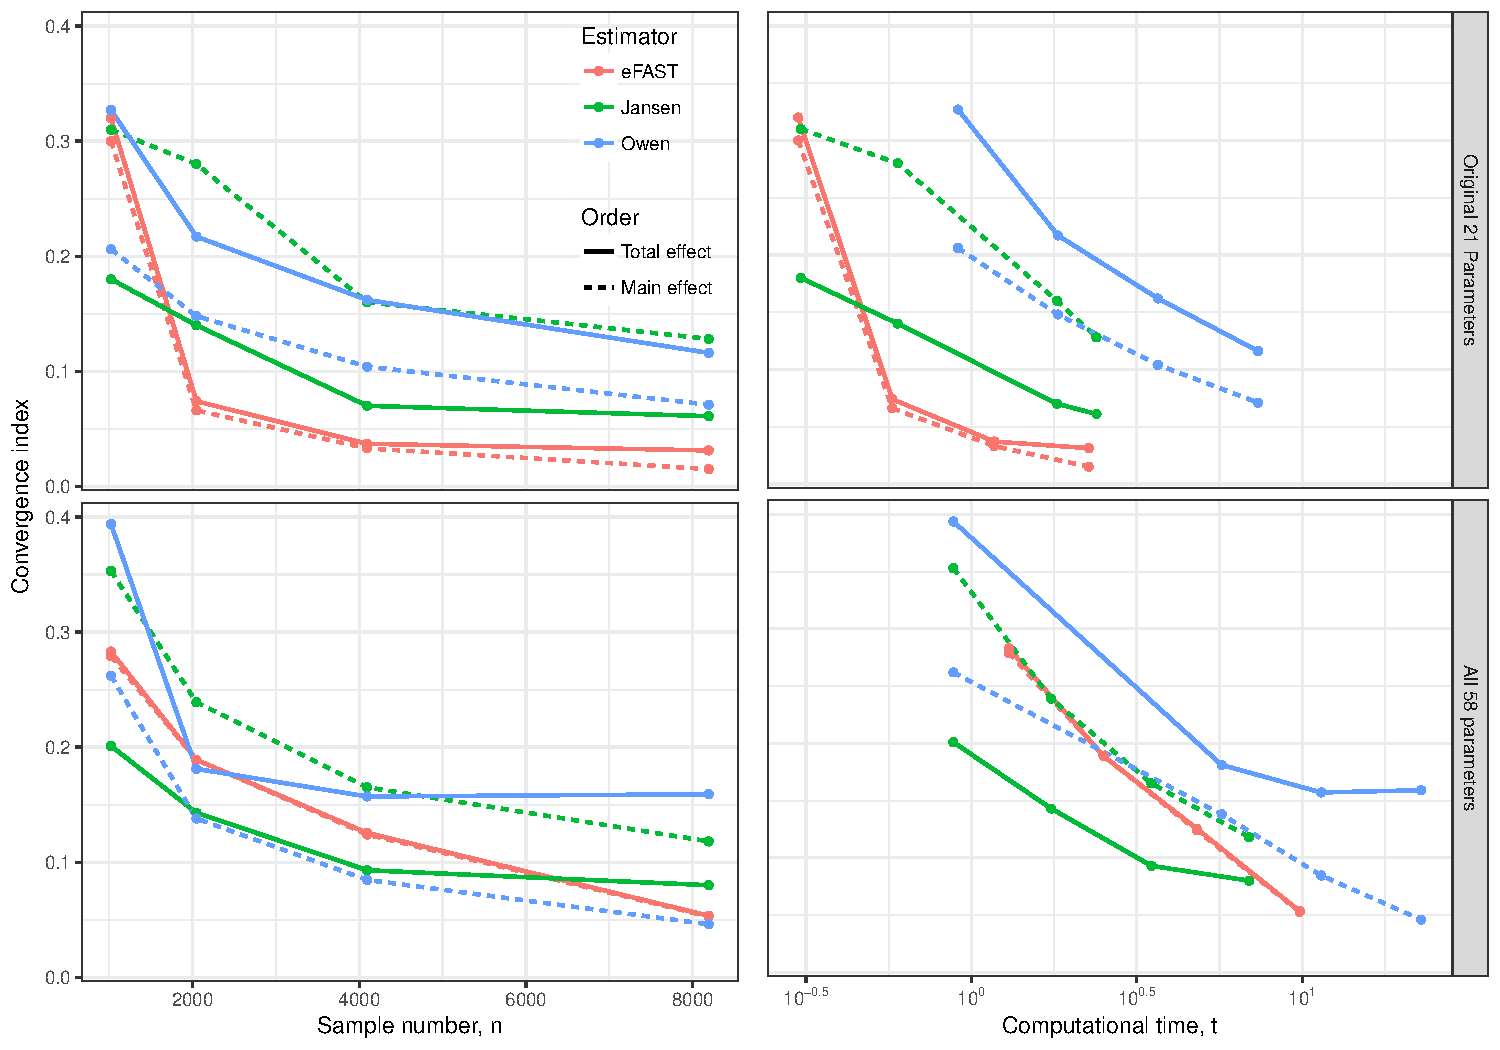
\includegraphics[width=0.98\linewidth]{fig2.pdf}
\caption{Illustration of the effect of model evaluation on convergence index and computation time (min).
The number of sample size has been increased up from 1024 to 8192 under original 21 and all 58 model parameter settings.
Under our setting range of sample size, the eFAST method can lead the expected convergence condition, resulting in convergence index less than 0.1.
}
\end{figure}
\end{block}


\begin{block}{Sensitivity Analysis for Original Model Parameter}
\begin{figure}
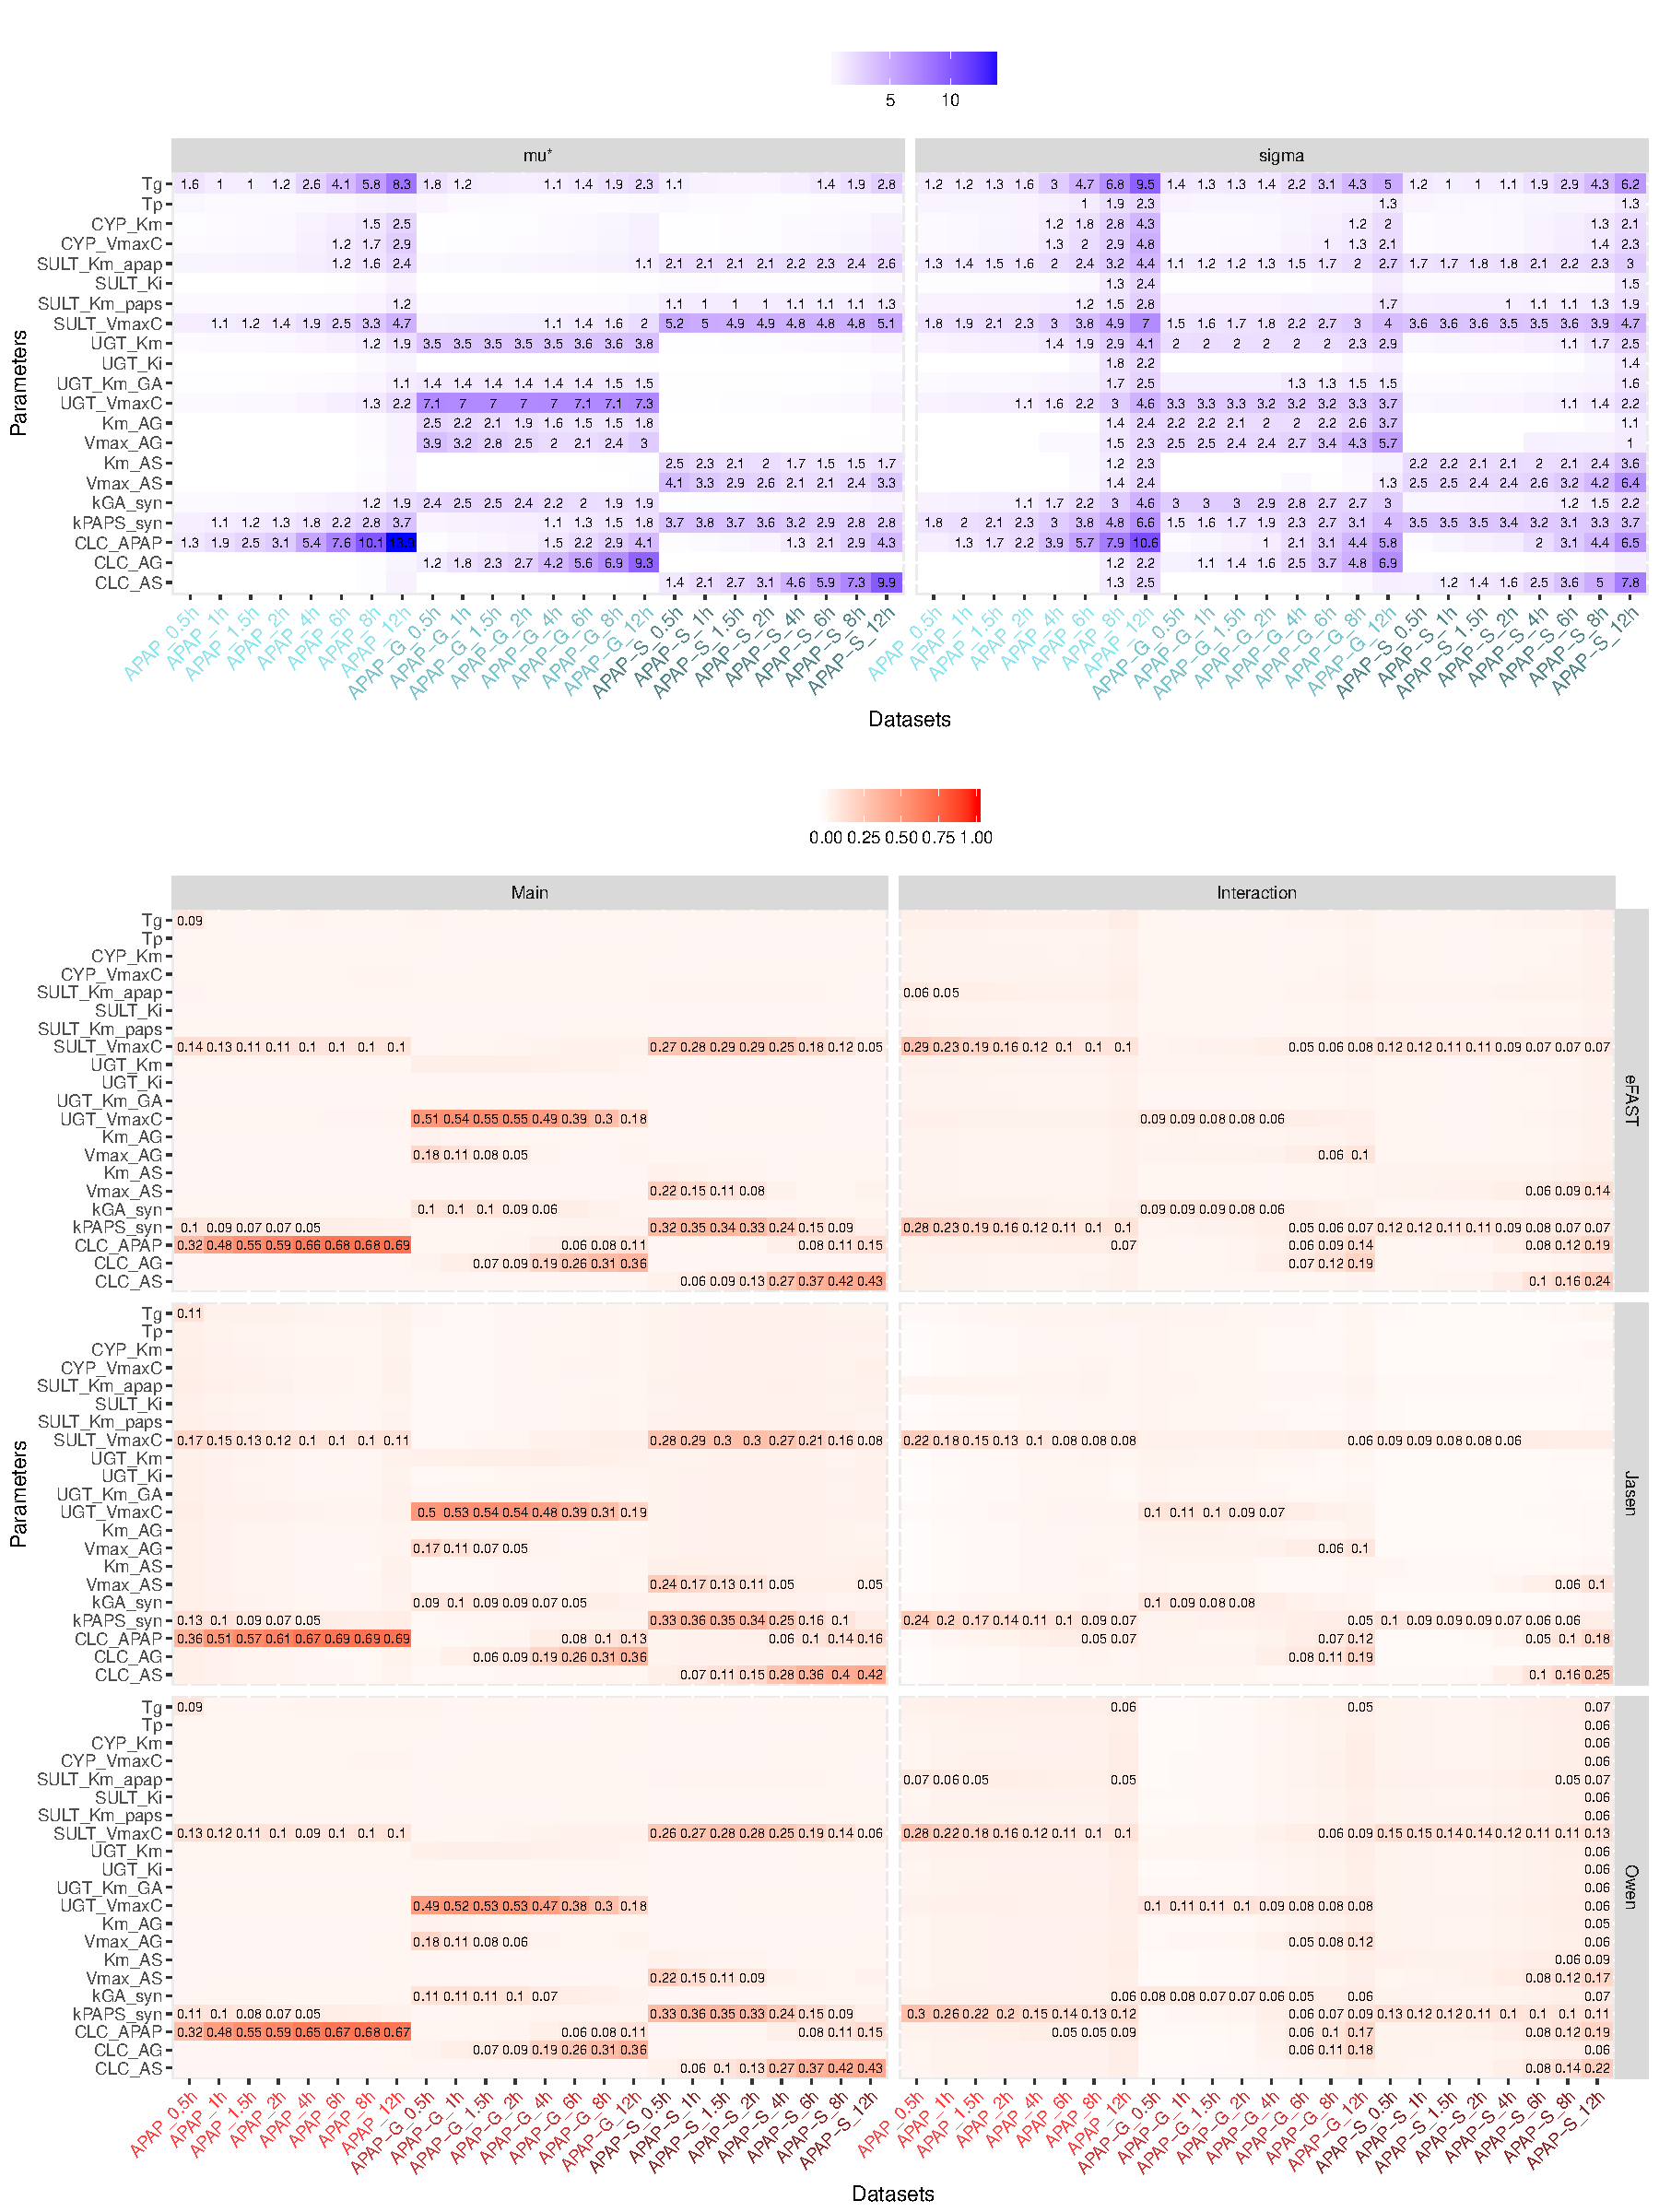
\includegraphics[width=0.98\linewidth]{fig3.pdf}
\caption{Time-dependent sensitivity coefficients computed through the different GSA methods with parent APAP and its conjugates. 
We can obtain that eFAST, Jansen, and Owen (variance-based method) can generate similar results. However, the sensitivity properties are different with Morris (one-step-at-a-time method).
According to the GSA result from eFAST, we found 11 parameters that influence the model output that Sobol indices were higher than the benchmark (0.05).
}
\end{figure}
\end{block}


\end{column} % End of the 2nd column

%%%%%%%%%%%%%%%%%%%%%%%%%%%%%%%%%%%%%%%%%%%%%%%%
\begin{column}{0.23\paperwidth} % The 3rd column
%
%
\begin{block}{Sensitivity Analysis for All Model Parameter}
\begin{figure}
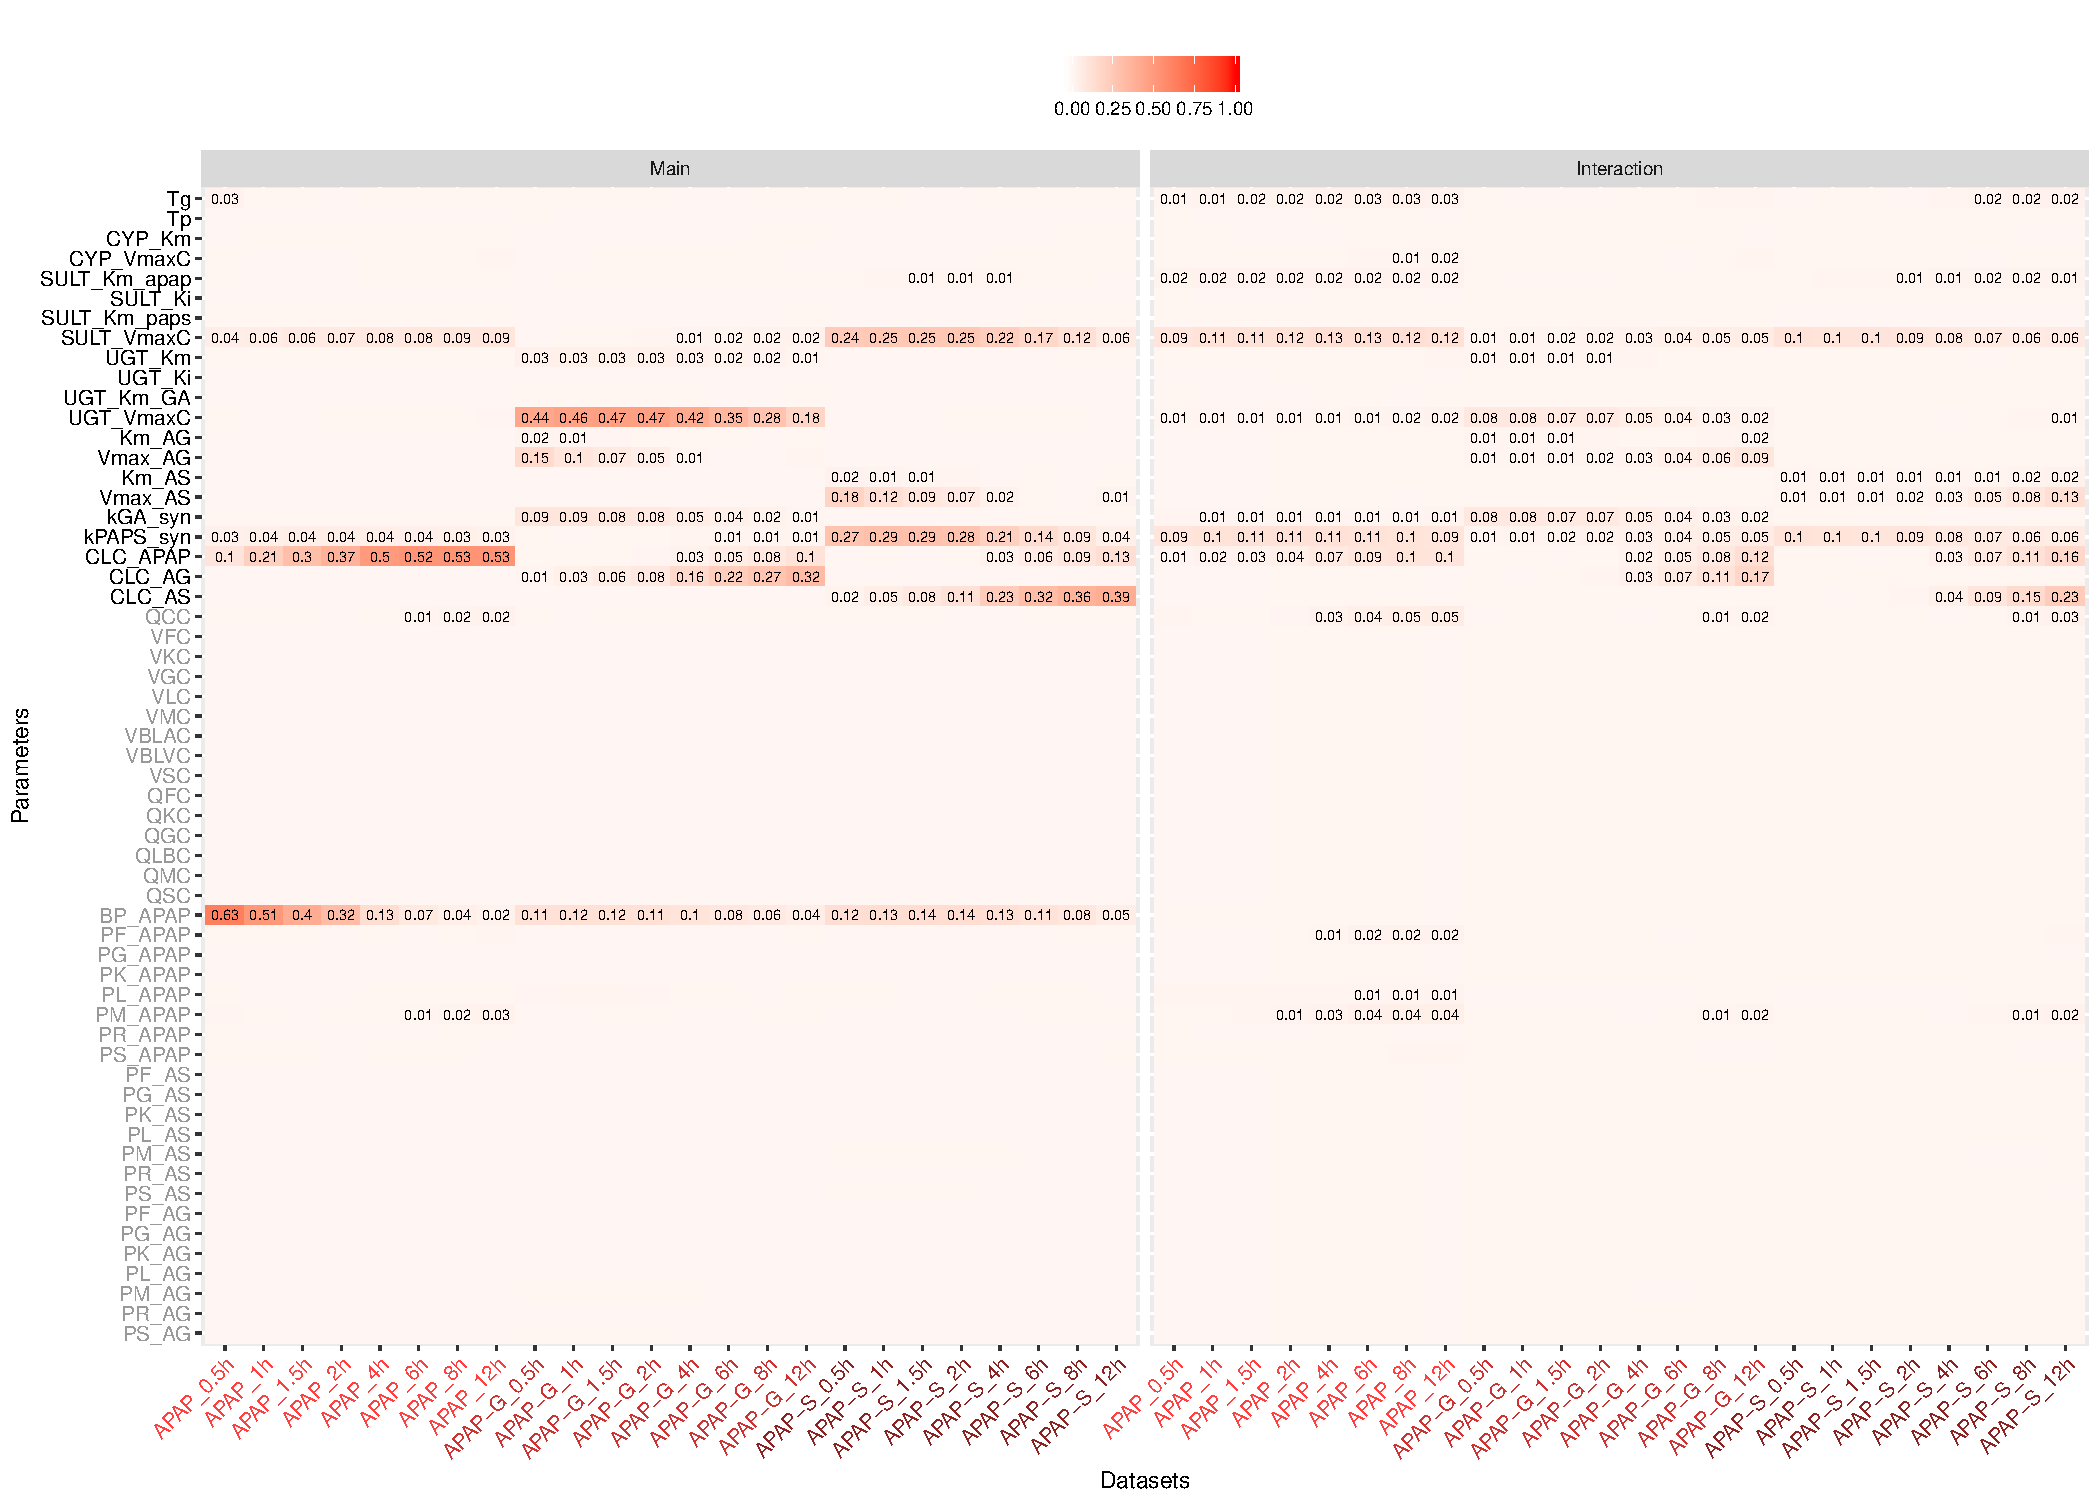
\includegraphics[width=0.98\linewidth]{fig5.pdf}
\caption{The result of sensitivity analysis of eFAST method that includes the original 21 original model parameters and 37 additional parameters that were fixed in the previous study. 
All 11 original sensitivity parameter still influence the model output. After incorporating the previously fixed parameters in our analysis, we further detect 9 parameters that Sobol indices were higher than the benchmark (0.01).}
\end{figure}
\end{block}
%
\begin{block}{Evaluation of Model Parameter}
\begin{figure}
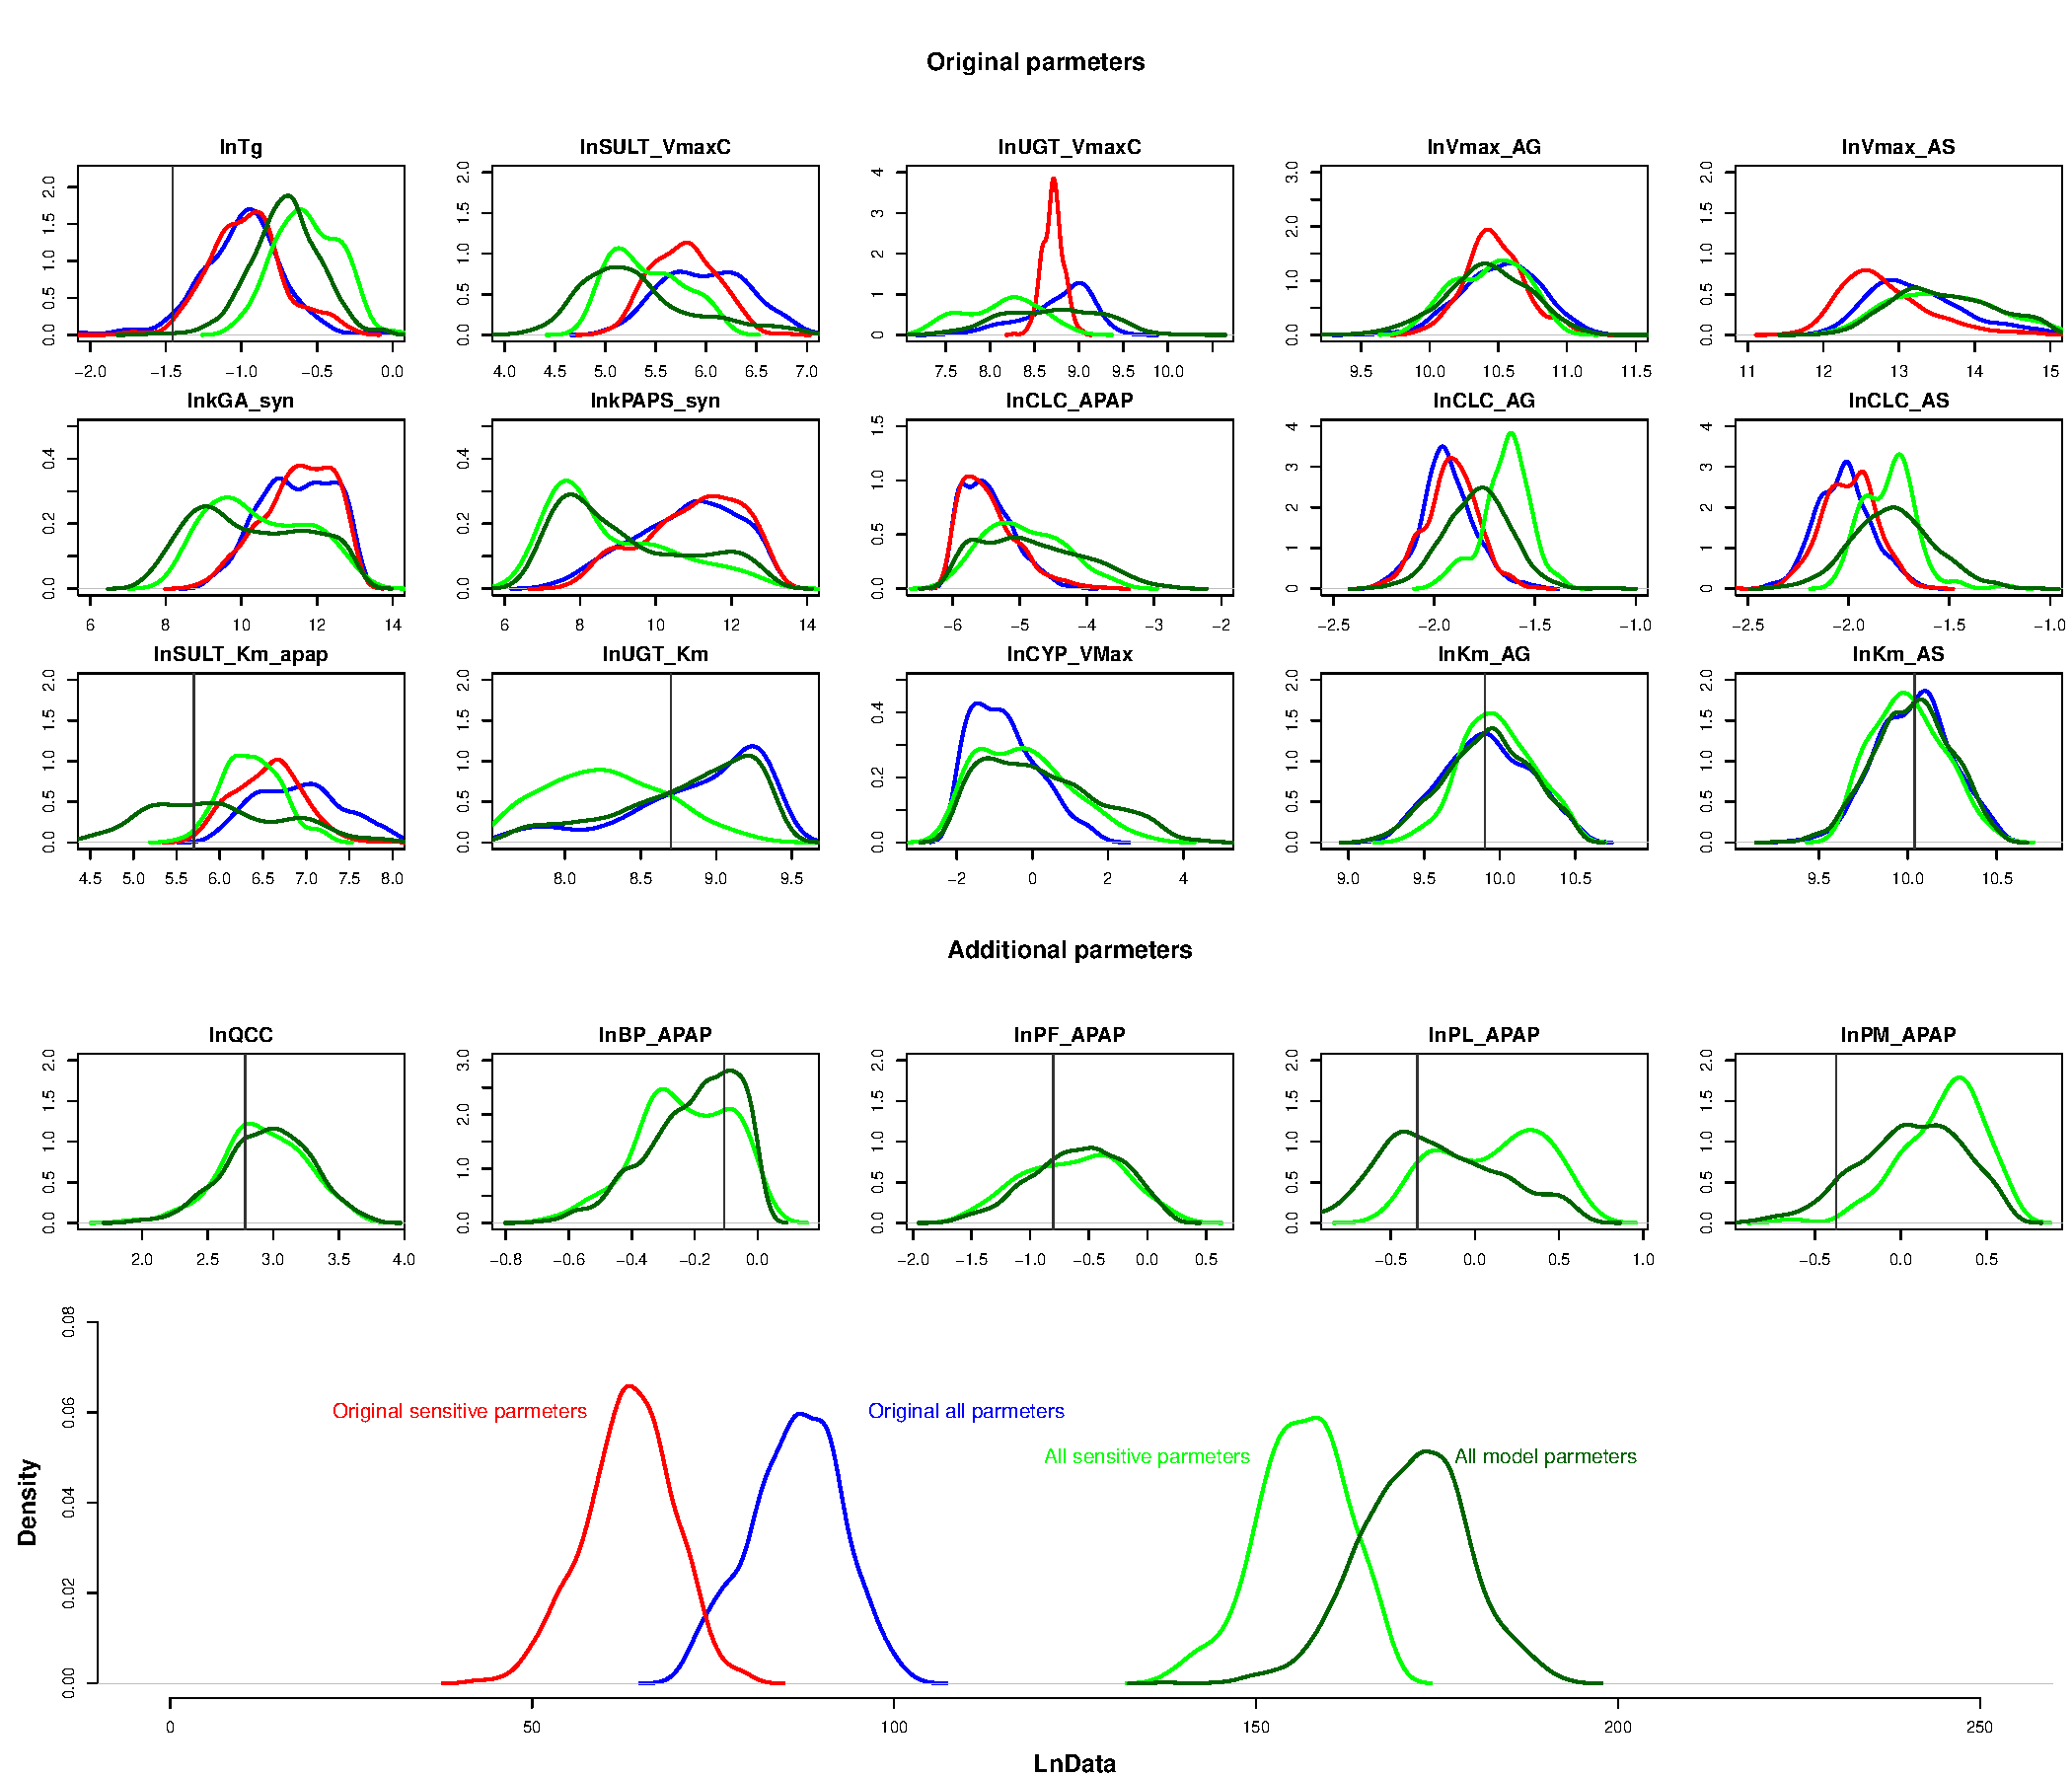
\includegraphics[width=0.98\linewidth]{fig6.pdf}
\caption{The comparison of the marginal posterior distribution of sensitive parameters and lndata. The result shows the statistical bias among four different parameter settings.
The result of lndata shows that the all model parameter setting has the best calibration result. 
Moreover, the current study can provide the better calibration result than original all parameter setting when only consider the sensitive parameter in PBPK model.
}
\end{figure}
\end{block}
 %
\begin{alertblock}{Conclusion}
\begin{itemize}
\item This study obtained the similar results from three different variance-based GSA methods.
\item Using eFAST method as GSA approach to determine which parameters to fix and which to estimate can lead to better computational efficiency.
\item The current approach can provide better model performance than the traditional judgment method.
However, we still need to clarify the reliable/robust benchmark that can use to do parameter screening.
\end{itemize}
\end{alertblock}
%
%
\end{column} % End of the 3rd column

%%%%%%%%%%%%%%%%%%%%%%%%%%%%%%%%%%%%%%%%%%%%%%%%%%
\begin{column}{0.22\paperwidth} % The 4th column
%
%
\begin{block}{Evaluation of Model Performance}
\begin{figure}
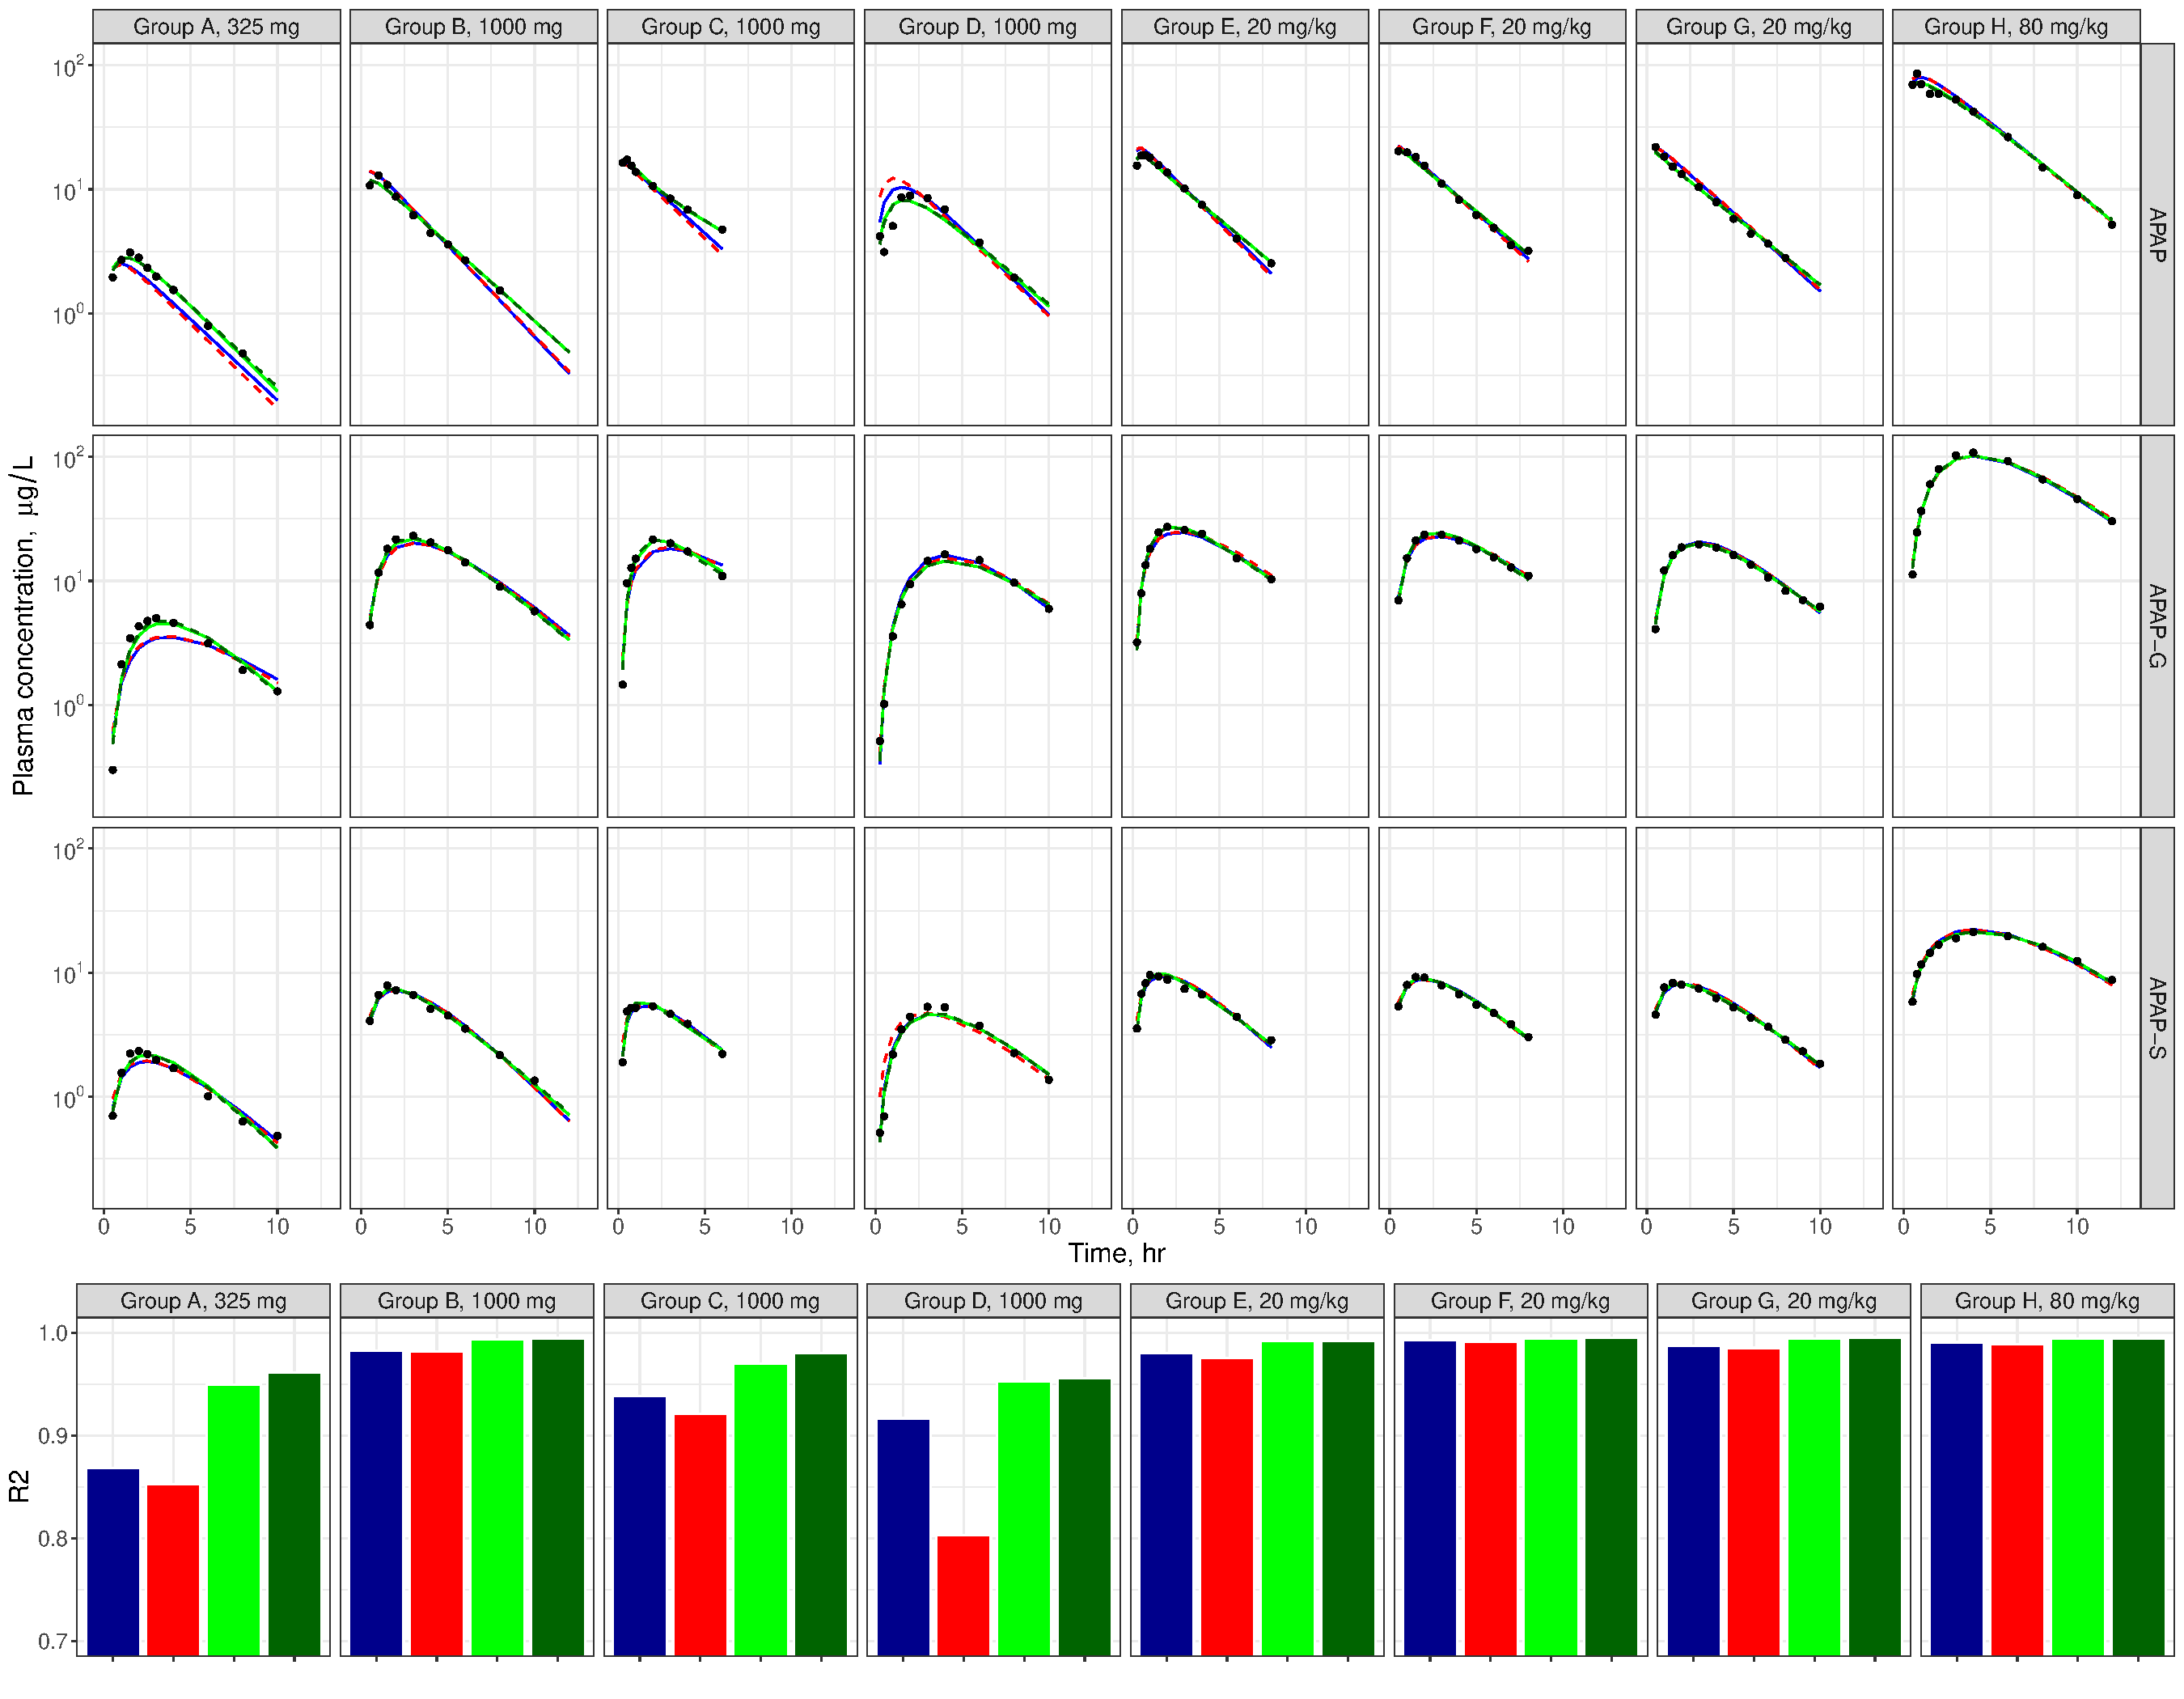
\includegraphics[width=\linewidth]{fig7.pdf}
\caption{Model evaluation result for the 8 experimental human studies with different APAP dosages. 
  The determination coefficient ($R^2$) was used to judge the model performance in each group.
}
\end{figure}
\begin{figure}
\begin{columns}
\column{.69\linewidth}
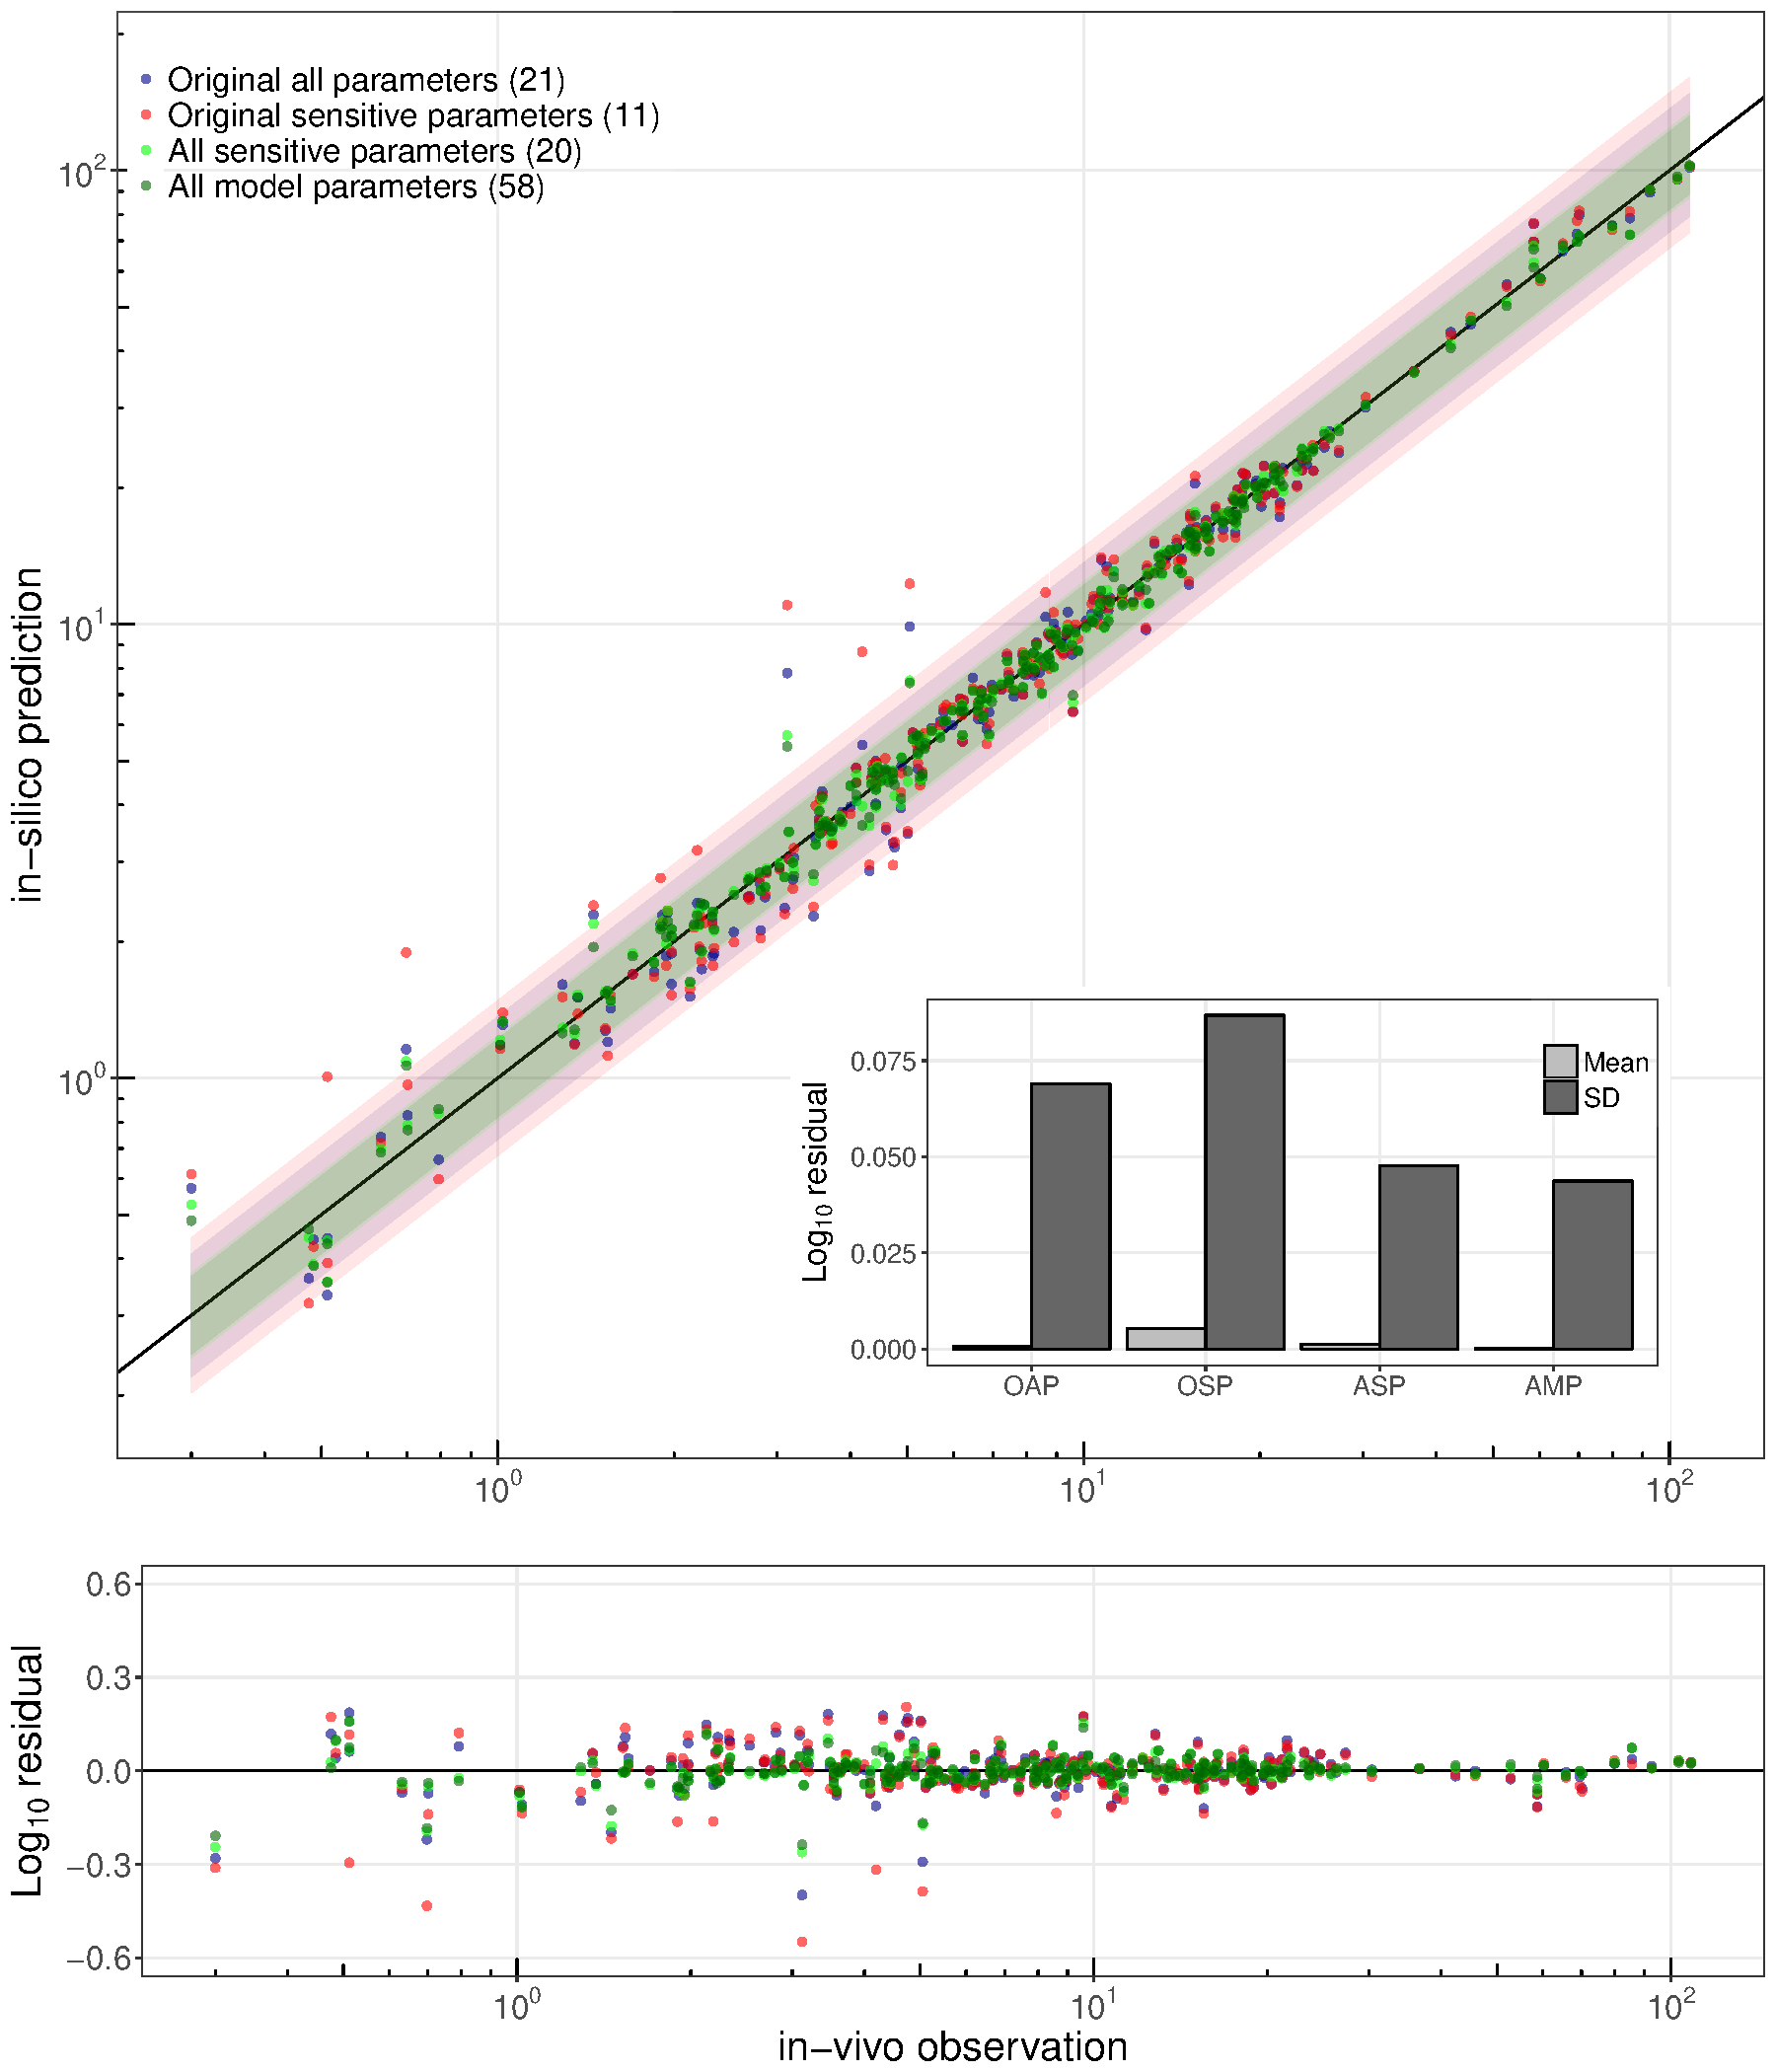
\includegraphics[width=\textwidth]{fig8.pdf}
\column{.30\linewidth}
\caption{Global evaluation of model fit and model performance. Restricting the MCMC simulation to the sensitive parameters can reduce computational burden while showing little change in model performance.
We further find that the simulation from all sensitive parameter (ASP) can provide better precision (residual SD) than original setting.
However, it cannot provide the same test result in accuracy (residual mean). }
\label{fig:example right}
\end{columns}
\end{figure}
%\begin{figure} % Do not use only [h] in real documents.
%\begin{minipage}{.67\linewidth}
%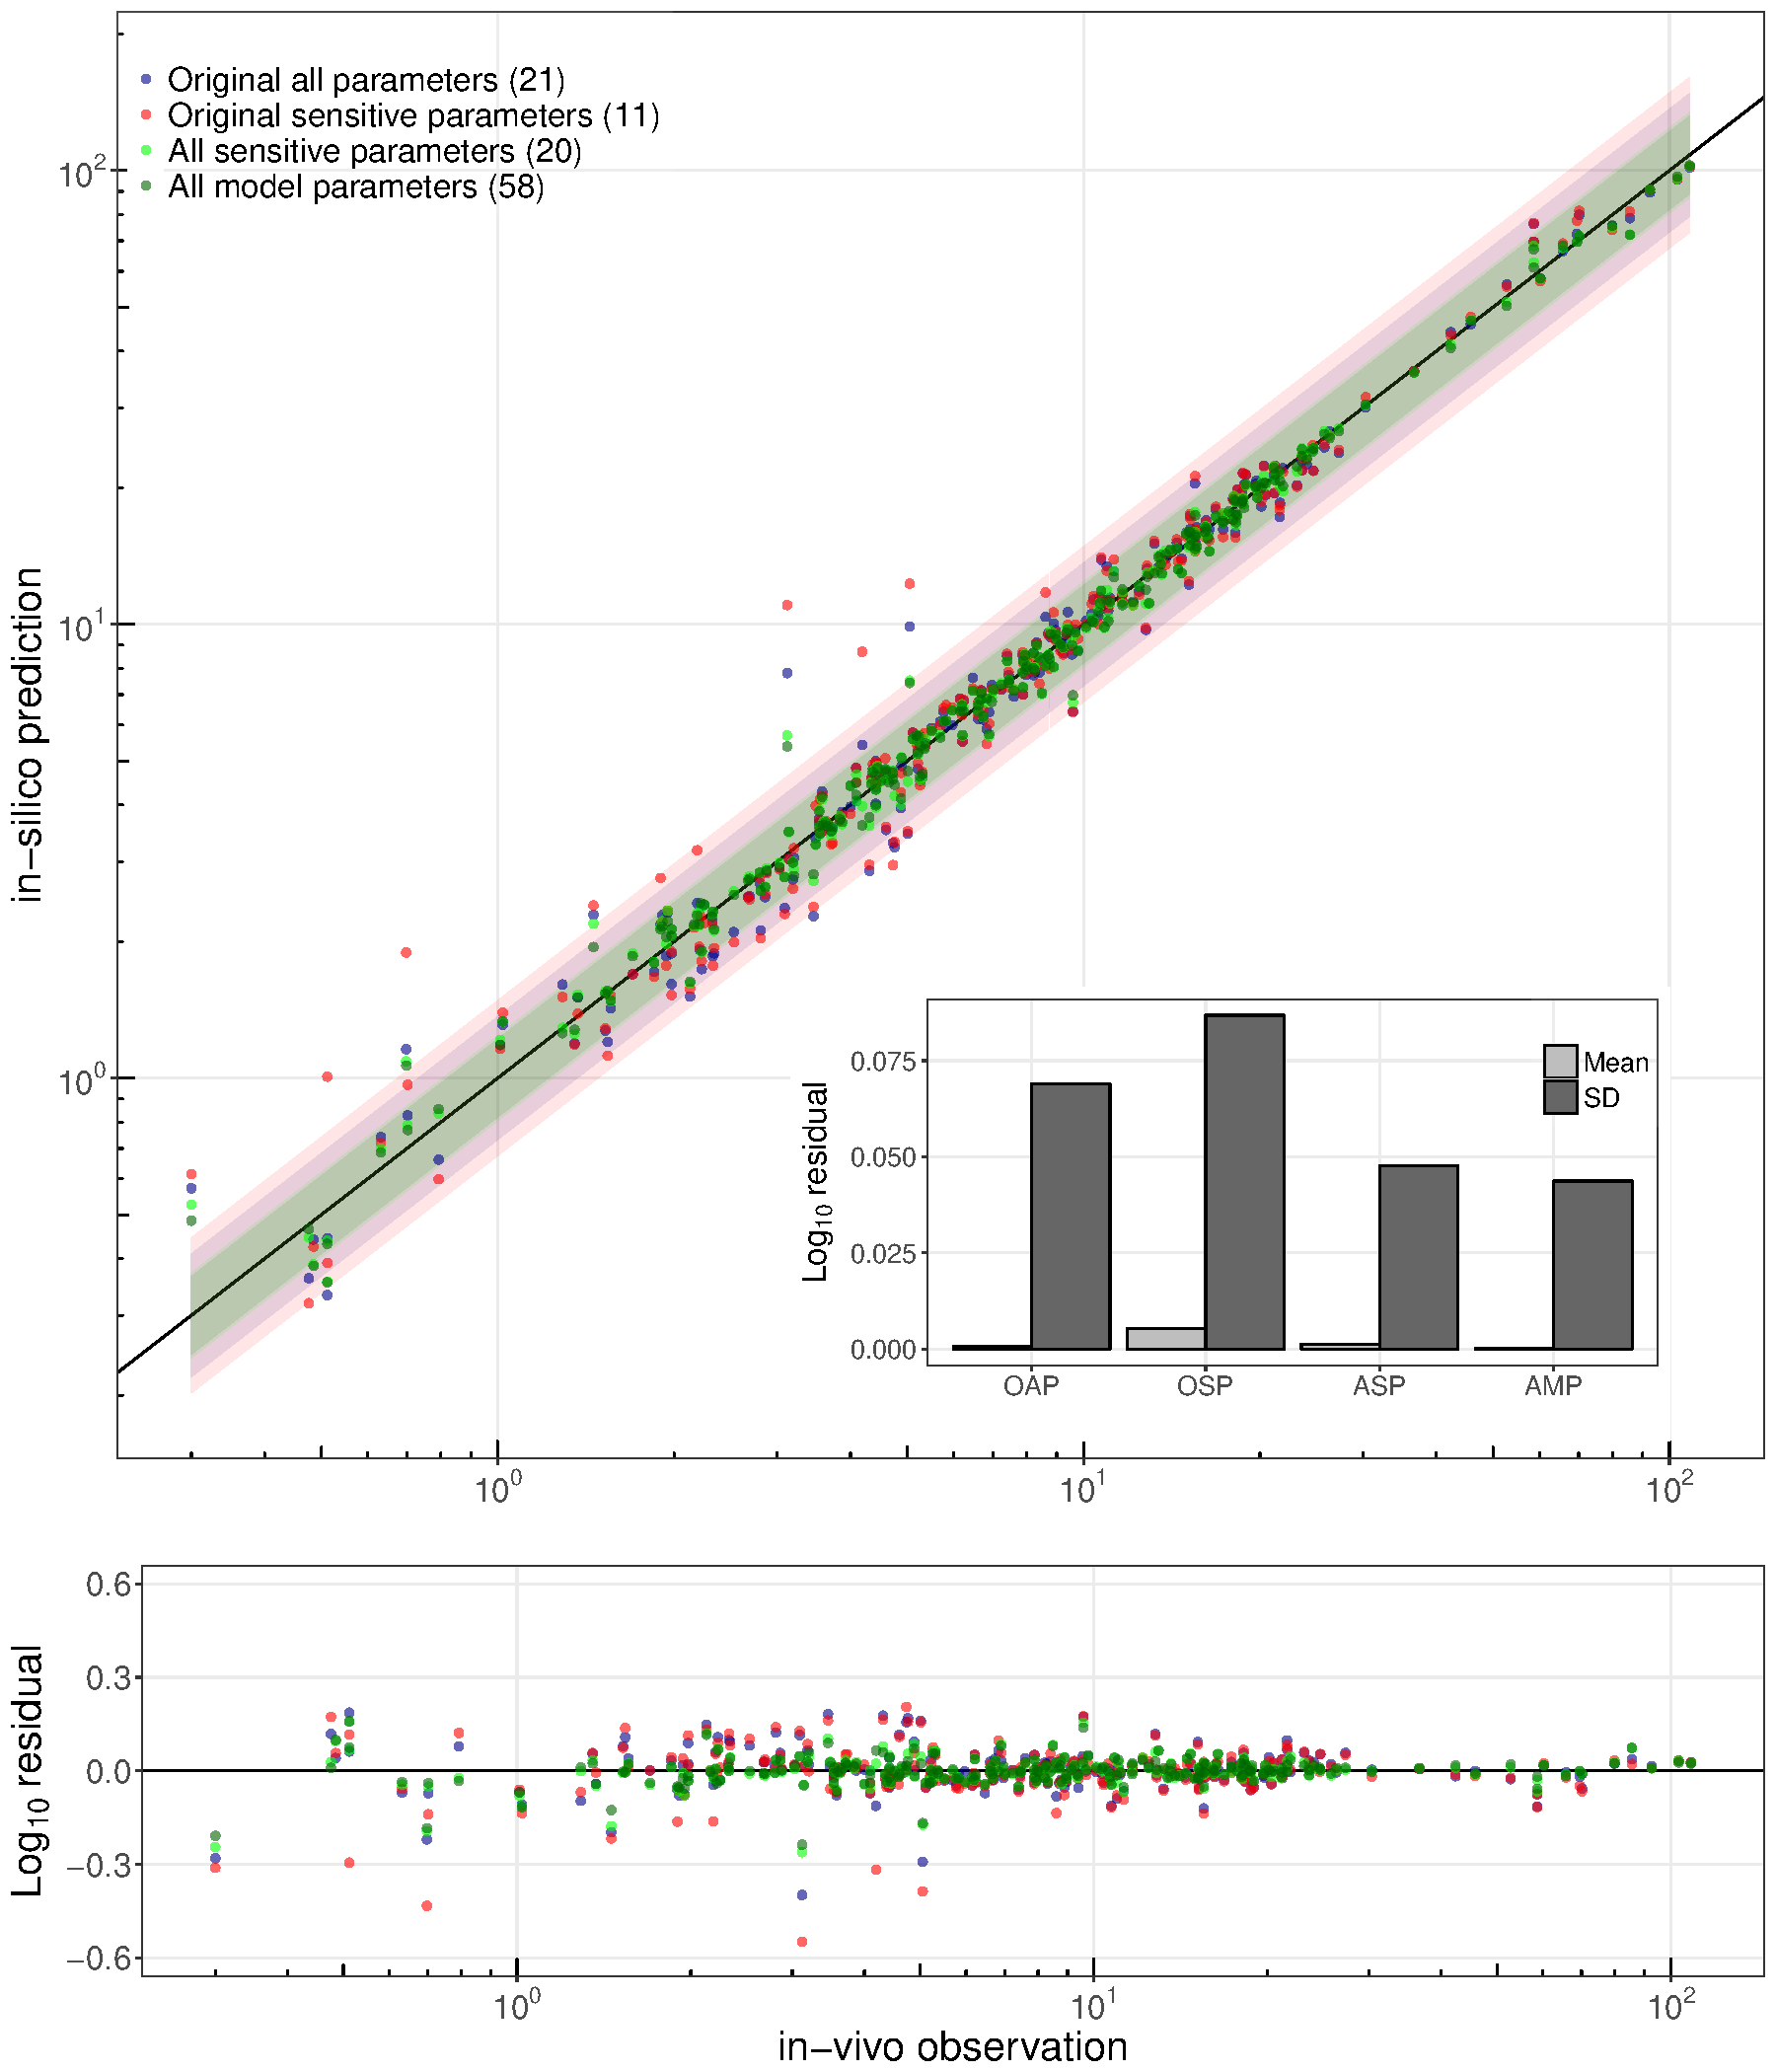
\includegraphics[width=\linewidth]{fig8.pdf}
%\caption{Global evaluation of model fit and model performance}
%\end{minipage}\hfill
%\begin{minipage}{.32\linewidth}
%Restricting the MCMC simulation to the sensitive parameters can reduce computational burden while showing little change in accuracy and precision in model performance.
%We further find that the simulation from all sensitive parameter (ASP) can provide better precision (residual SD) than original setting.
%However, it cannot provide the same test result in accuracy (residual mean). 
%\end{minipage}
%\end{figure}
\end{block}
%
\begin{block}{The Computational Efficiency for GSA and MCMC}
\begin{table}
\begin{adjustbox}{max width=\textwidth}
\begin{threeparttable}
  \centering
  \caption{Summary of parameter and computational time cost for GSA (n=8,192) and MCMC (n=300,000)}
  \label{tab:table1}
  \rowcolors{2}{Maroon!15}{white}  
  \begin{tabular}{llcccc}
  \rowcolor{Maroon!30}   
    \toprule
    &  & All parameter & Original estimated & All sensitive & Original sensitive \\
    \midrule
    \multicolumn{2}{l}{Number of parameter} & 58 & 21 & 20 & 11 \\
    \multicolumn{2}{l}{MCMC (hr)} & 20.8 & 35.2 & 37.1 & 66.3 \\
	    GSA (min) & eFAST & - & - & 2.26 & 9.83 \\
	   \multirow{2}{*}{} & Jansen & - & - & 2.39 & 6.91 \\
	    & Owen & - & - & 7.3558 &  22.89 \\
    \hline   
  \end{tabular}
   \end{threeparttable} 
   \end{adjustbox}
\end{table}
\end{block}
%
\setbeamercolor{block title}{fg=red,bg=white} % Change the block title color
\begin{block}{Acknowledgements}
\small This work was supported by U.S. Food and Drug Administration (RFA-FD-16-026) \\
\end{block}
%
\begin{alertblock}{Bibliography}
\begin{thebibliography}{9}
{\footnotesize \bibitem{Zurlinden}
Zurlinden TJ and Resifeld B. (2016) Eur J Drug Metab Pharmacokinet, 41:267-80.}
{\footnotesize \bibitem{McNally}
McNally K et al. (2011) Front Pharmacol 2:31.}
{\footnotesize \bibitem{Jansen}
Jansen MJW (1999) Comput Phys Commun 117:35-43.}
{\footnotesize \bibitem{Owen}
Owen AB (2013) ACM Trans Model Comput Simul 23(2).}
{\footnotesize \bibitem{Pujol17}
Pujol G. (2017) Sensitivity analysis. Package "Sensitivity", CRAN Repository.}
{\footnotesize \bibitem{Bois09}
Bois FY (2009) Bioinformatics 25: 1453-1454.}
\end{thebibliography}
\end{alertblock}

%----------------------------------------------------------------------------------------

\end{column} % End of the third column

\end{columns} % End of all the columns in the poster

\end{frame} % End of the enclosing frame

\end{document}
